\chapter{Multiple Input Multiple Output Line Of Sight Channel}

this system uses a multiple antennas at the \Tx and \Rx to decrease the probability of error in the communication system, and that's a type of Spatial Diversity.

\section{\Tx \& \Rx antenna arrays}
we already defined those arrays in MISO and SIMO systems, we we will just call them back again.


\subsection{Scatteringchanmtx}
as we did in SISO, SIMO and MISO LOS, we will repeat it for this system because we need scattering channel matrix to calculate the BER.
the difference here is we will place the antenna array we made at both \Tx and \Rx.

\section{Bit Error Rate (BER)}
we will calculate it this time for the MIMO system.

to monitor the relationship between Eb/No and BER in a MIMO LOS channel so will use the 11 values of Eb/No and calculate the BER for each one using helpMIMOBER function.

\vfill
\begin{figure}
	\centering
	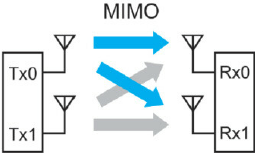
\includegraphics[width=0.4\linewidth]{figures/MIMO}
	\caption{MISO}
\end{figure}


\newpage
\section{Plotting}
to see the difference between SISO, SIMO (or MISO) and MIMO we will plot all of them on the same graph.

as we can see in Figure[\ref{fig:sisosimomimober}], the BER decreases as we increase the Eb/No for each SISO, SIMO and MIMO.


\begin{figure}[!h]
	\centering
	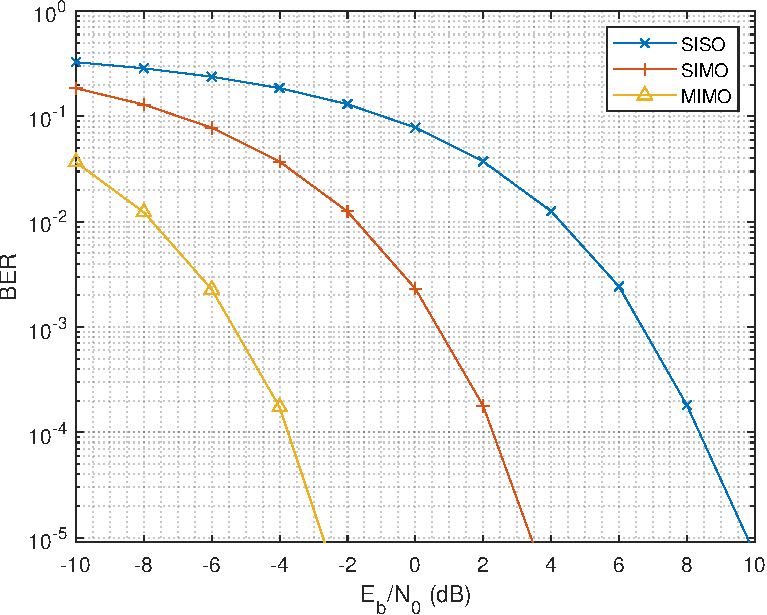
\includegraphics[width=1\linewidth]{figures/SISO_SIMO_MIMO_BER}
	\caption{}
	\label{fig:sisosimomimober}
\end{figure}



\newgeometry{margin=0pt}
\newpage
\vfill
\begin{figure}
	\centering
	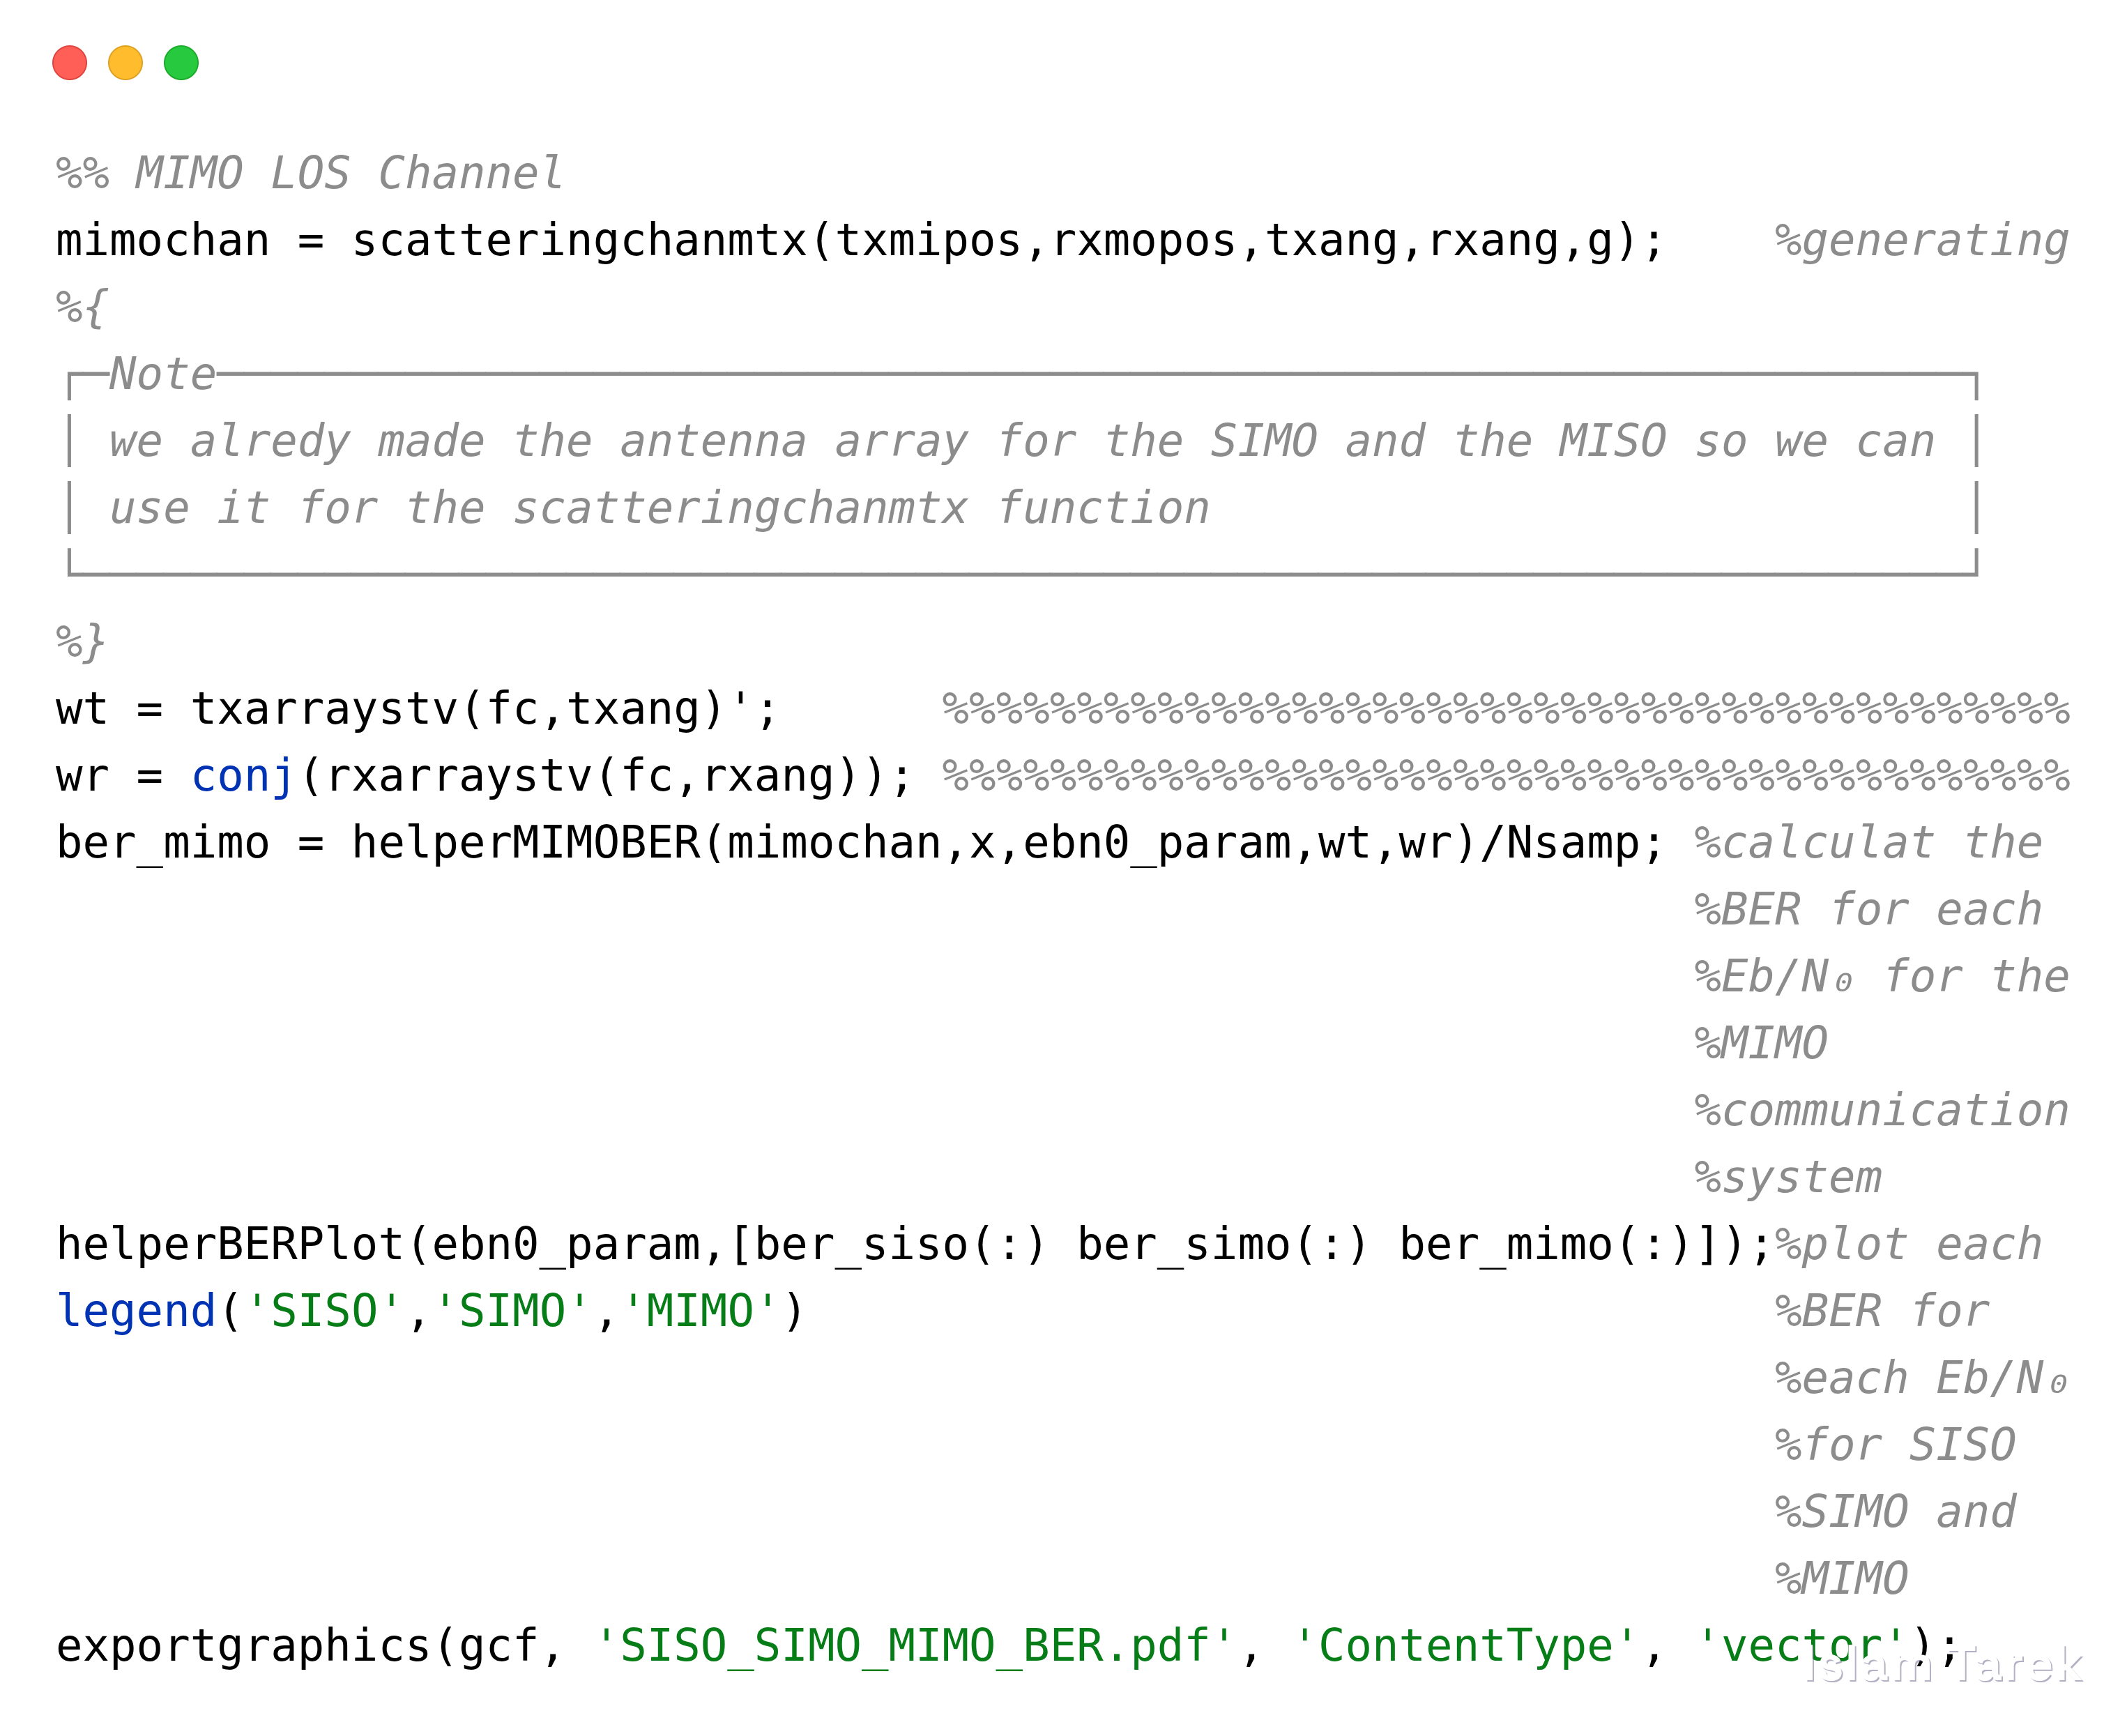
\includegraphics[width=0.7\linewidth]{figures/code5}
\end{figure}
\vfill
\restoregeometry